\section{Simulation Results: P1--P4}
\label{sec:results14}
All results in this section are \lvl{L1} (floating point, Gaussian noise), supervised unless stated, with the parameters of \cref{tab:params}.

\subsection{P1: validation of the apparatus}
\label{sec:p1}
Before any tracking result, the PPR required the flat-channel BER against theory, the static-ISI error floor and its removal, convergence to the Wiener filter, the choice of $\Delta$ and the check of the training sequence. \nb{On a flat channel the BER at 12 SNR points ($2\times10^6$ bits each) lies on $Q(\sqrt{2E_b/N_0})$, with 11 of 12 points inside their 95\,\% interval and all 12 inside 99\,\% (\cref{fig:p1}a); this checks noise scaling, threshold, SNR definition and bit counting together. On static ISI channels R1 has an error floor (14--20\,\% at $a=0.91$ at every SNR) that matches its exact analytic BER, and R2/R3 remove it (no errors in $10^6$ bits at 16\,dB; \cref{fig:p1}b). LMS converges to the Wiener filter (average coefficients within 0.17--0.18\,\%), the oracle agrees with a brute-force computation to 0.32\,\%, and the bit-alignment, PRBS and noise tests pass. One test fails: the textbook misadjustment.}

\begin{figure*}[t]
\centering
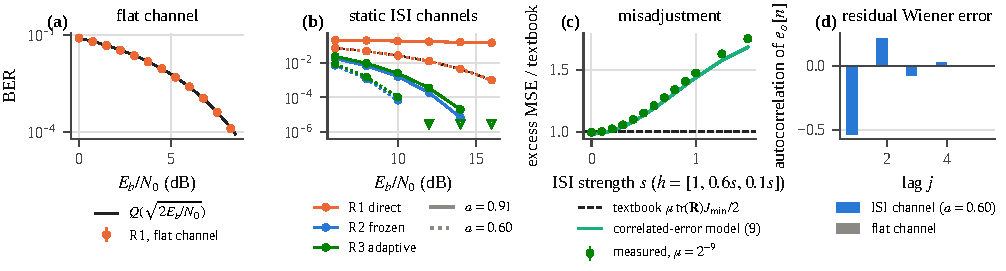
\includegraphics[width=\linewidth]{figs/p1.pdf}
\caption{P1 validation (\lvl{L1}). (a)~Flat-channel BER of the direct detector against BPSK theory. (b)~Static ISI channels ($a=0.91$ solid, $0.60$ dotted): R1 against its exact BER (black), and R2, R3. \nb{Triangles: no errors observed (plotted at the 95\,\% upper bound). (c)~Measured excess MSE divided by the textbook misadjustment, against ISI strength, with the correlated-error model \eqref{eq:corrmis}; the textbook value holds only on a flat channel. (d)~Autocorrelation of the Wiener filter's residual error: strongly negative at lag 1 on the ISI channel, zero on a flat channel.}}
\label{fig:p1}
\end{figure*}

\subsubsection*{\nb{Correction of the misadjustment formula}}
\label{sec:misadj}
\nb{On the control channel ($a=0.60$, 14\,dB) the measured excess MSE is \textbf{1.47--1.48 times} $\mu\,\mathrm{tr}(\mathbf R)J_{\min}/2$ (16 independent seeds of $10^6$ symbols, 95\,\% intervals $\pm0.003$), while on a white-input flat channel the same measurement matches the formula within 1--3\,\% and halves when $\mu$ halves. The formula assumes that the error $e_o$ left by the optimum filter is white and independent of the input. On an ISI channel that residual is mostly leftover interference, so neighbouring errors are strongly correlated (lag-1 correlation $-0.53$, \cref{fig:p1}d). Keeping that correlation in the first-order analysis gives
\begin{equation}
\begin{aligned}
\xi_{\rm ex}&\approx\tfrac{\mu}{2}\Big(C(0)-2\textstyle\sum_{j\ge1}C(j)\Big),\\
C(j)&=E\big[e_o[n]\,e_o[n-j]\,\mathbf u^T[n]\mathbf u[n-j]\big],
\end{aligned}
\label{eq:corrmis}
\end{equation}
where $C(j)$ is computed exactly from the channel, without simulation. Here $C(0)=0.606$ equals $J_{\min}\mathrm{tr}(\mathbf R)$ within 0.6\,\%, but $\sum_{j\ge1}C(j)=-0.144$, so \eqref{eq:corrmis} predicts $(0.606+0.288)/0.609=1.468$ times the textbook value, against 1.468--1.480 measured. Shuffling the data in time, which removes the correlation, restores the textbook value (ratio 0.99--1.00). Widrow \etal already observed measured misadjustment 1.2--1.9 times above the formula in their adaptive predictor and attributed it to correlated input samples \cite[Table~I]{widrow1976}; \eqref{eq:corrmis} turns that observation into a prediction. Over ISI strength the ratio rises from 1.00 (flat) to 1.75 ($a=0.90$), and \eqref{eq:corrmis} follows it within 1.5--4\,\% (\cref{fig:p1}c). The textbook form is therefore an incorrect use of an approximation here, not a simulation error, and \eqref{eq:corrmis} is used for all predictions in this report.}

\noindent\textbf{Decision delay and alignment.} The PPR expected a clear MSE minimum against $\Delta$ and a large difference between a non-minimum-phase channel and its mirror. \nb{For $h=[0.5,1.0]$ the Wiener MSE at $\Delta=0$ is 0.756 (LMS 0.797) against 0.025 at the best delay ($\Delta\approx6$--11, flat); for the mirror $[1.0,0.5]$ it is 0.026 at $\Delta=0$ (\cref{fig:delay}). Identical magnitude responses give a factor of 30 in MSE, and LMS follows the Wiener curve at every $\Delta$, about 5\,\% above it. On the project channels the best $\Delta$ is 3--7 (primary) and 5--7 (control), but the minimum is so flat that the fixed $\Delta=2$ costs at most 1.3\,\% MSE, and only 0.07--0.27\,\% on the moving channel; $\Delta$ therefore need not follow the channel. The cross-correlation peak equals the predicted offset for every receiver (lag 0 for R1, 2 for R2 and R3); a wrong offset gives BER 0.499--0.503.}

\begin{figure}[t]
\centering
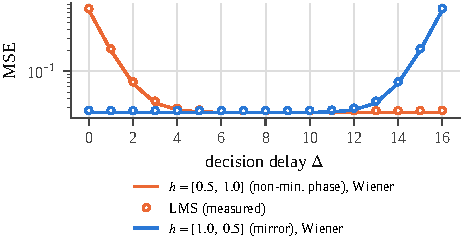
\includegraphics[width=\linewidth]{figs/delay.pdf}
\caption{Decision-delay sweep for the non-minimum-phase preset $h=[0.5,1.0]$ and its mirror, 14\,dB (\lvl{L1}): Wiener MSE (lines) and measured LMS (circles). \nb{The two channels have the same magnitude response; the non-minimum-phase one needs $\Delta\ge5$.}}
\label{fig:delay}
\end{figure}

\subsection{P2: abrupt transitions and reacquisition}
\label{sec:p2}
The MSE around each step (\cref{fig:p2}) and $N_{\rm rec}$ against $\mu$ (\cref{fig:nrec}) were planned to show reacquisition. R3 reacquires while R2 stays at the mismatched level. \nb{The recovery time is inversely proportional to the step size: the log--log slopes of $N_{\rm rec}$ against $\mu$ are $-1.06/-1.00/-0.98$ at 16\,dB and $-1.03/-1.02/-0.97$ at 14\,dB for the three steps, against $-1.07\ldots-1.00$ from the noise-free mean-weight model $E[\mathbf w]=\mathbf w_B+(\mathbf I-\mu\mathbf R_B)^k(\mathbf w_A-\mathbf w_B)$. On the harsh step the measured value lies above the model (e.g.\ 3386 against 3067 symbols at $\mu=2^{-8}$), the expected one-sided bias of a last-crossing statistic, and individual values there are uncertain by about $\pm20$\,\%. R2 after the step matches its analytic frozen-filter MSE (e.g.\ 0.395 against 0.393).}

\nb{\emph{Training length.} With $N_T=60000$, R2 after the ``down'' step was 0.7--3.0\,\% \emph{better} than an ideally trained filter. The mean-weight model predicted why: the slowest direction of $\mathbf R$ ($\lambda_{\min}\approx0.07$ at $c=116$) still held about 1\,\% weight error after 60000 symbols, invisible on the training channel. With $N_T=120000$ the offset fell to $-0.6\ldots+0.05$\,\% (at $\mu=2^{-10}$: $-2.31\to+0.05$\,\%, model $-2.10\to\approx0$). Small residual offsets (up to $+1.7$\,\% at 14\,dB, $\mu=2^{-7}$, falling with $\mu$) remain \emph{unexplained} and are reported as measured; the $N_T=60000$ results are preserved.}

\begin{figure*}[t]
\centering
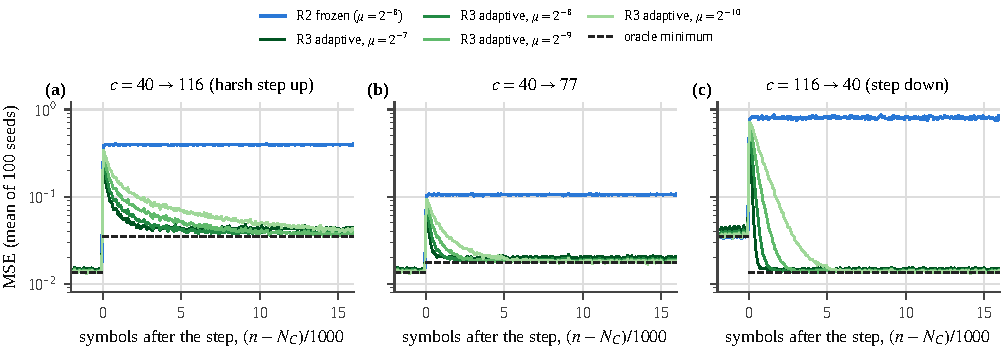
\includegraphics[width=\linewidth]{figs/p2.pdf}
\caption{Abrupt transitions at $N_C$, primary channel, 16\,dB, 100 seeds, $N_T=120000$ (\lvl{L1}): MSE against time for R2 and for R3 at four step sizes; dashed: oracle minimum before and after the step. \nb{R3 reacquires, faster for larger $\mu$; R2 stays at the mismatched level.}}
\label{fig:p2}
\end{figure*}

\begin{figure}[t]
\centering
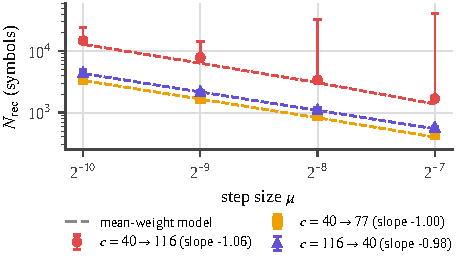
\includegraphics[width=\linewidth]{figs/p2nrec.pdf}
\caption{Reacquisition time $N_{\rm rec}$ against $\mu$ for the three steps, 16\,dB, 100 seeds (\lvl{L1}): measured (95\,\% seed bootstrap) and mean-weight model (dashed). \nb{All three follow $N_{\rm rec}\propto1/\mu$; the wide intervals on the harsh step come from the noisy last-crossing statistic.}}
\label{fig:nrec}
\end{figure}

\subsection{P3: tracking against the variation rate}
\label{sec:p3}
The PPR's principal result is the BER of R1, R2 and R3 against the variation rate on identical data (\cref{fig:ber}). R1 and R2 are flat, because they never adapt and every evaluation window covers whole up-and-down periods, so they see the same mix of channel states at every speed; only R3's error depends on speed, which is what the experiment isolates. R3 holds its static BER at slow variation and rises towards a ceiling at fast variation.

\begin{figure*}[t]
\centering
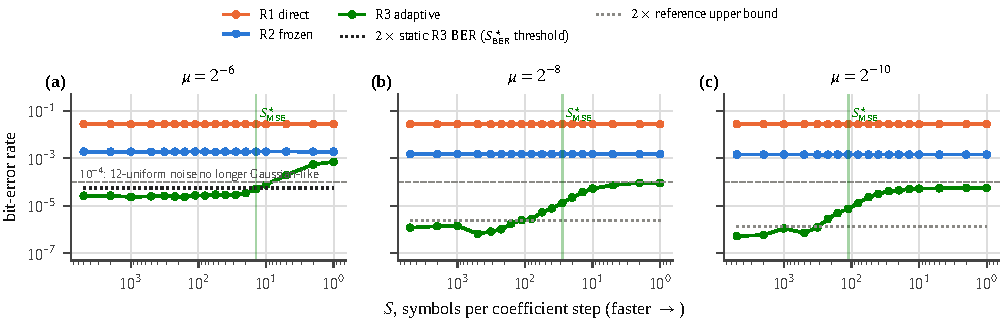
\includegraphics[width=\linewidth]{figs/ber_vs_S.pdf}
\caption{BER against variation rate for R1, R2 and R3, primary channel, 14\,dB, 100 seeds (\lvl{L1}, Gaussian noise). Dotted: the $S^\star_{\rm BER}$ threshold, $2\times$ the static R3 BER. Dashed: $10^{-4}$, below which the planned 12-uniform hardware noise no longer approximates Gaussian BER (\cref{sec:channel}); these \lvl{L1} curves use Gaussian noise. \nb{Green line: $S^\star_{\rm MSE}$. R3 loses BER at slower rates as $\mu$ falls; it stays below R2 at every rate for these $\mu$.}}
\label{fig:ber}
\end{figure*}

\nb{\emph{MSE boundary.} The tracking loss $\rho$ rises from 0 to about 1 as $S$ falls (\cref{fig:rho}). $S^\star_{\rm MSE}$ is bracketed inside the grid in all 68 cases where $\rho$ is defined, and never shows a pass after a non-pass. For $\mu\le2^{-7.5}$ it is the same on both channels at 14 and 16\,dB (within one grid step at 12\,dB) and doubles each time $\mu$ halves: $S^\star_{\rm MSE}\cdot\mu=0.109$--0.110 (\cref{fig:bound}a, \cref{tab:sstar}). At larger $\mu$ the static misadjustment uses up part of the room below the plateau and the boundary flattens; at $\mu=2^{-5}$, 12--14\,dB, $\rho$ is undefined. \Cref{sec:theory} derives this law.}

\nb{\emph{What the boundary means.} $S$ is the number of symbols between successive one-step changes of the channel coefficient, so a smaller $S$ is a faster-changing channel. $S^\star_{\rm MSE}$ is the fastest rate on the tested grid at which R3's tracking loss is still statistically below half of the way to a fixed filter (\cref{sec:metrics}). The law $S^\star_{\rm MSE}\approx0.11/\mu$ says that, within the tested regime, \emph{halving the step size requires doubling the number of symbols between channel changes} --- the channel must change half as often --- to keep the same tracking accuracy: a smaller step averages out more noise but adapts proportionally more slowly. The law is measured for these two channels, $L=16$, 12--16\,dB and $\mu\le2^{-7.5}$; it is not a universal property of adaptive equalizers or of physical channels, and at larger $\mu$ the static misadjustment bends it (\cref{fig:bound}a).}

\begin{figure*}[t]
\centering
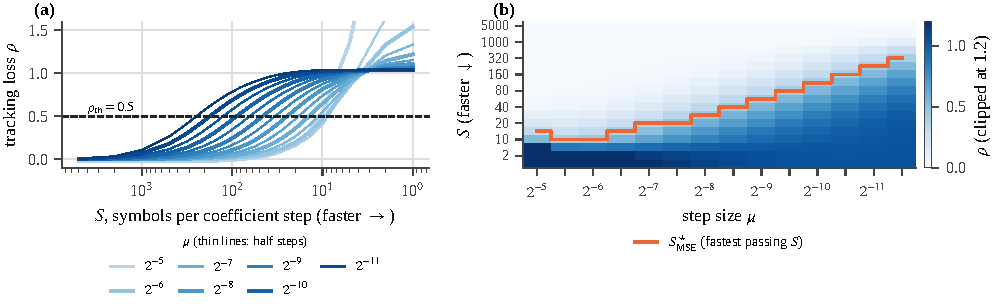
\includegraphics[width=\linewidth]{figs/rho.pdf}
\caption{\nb{Tracking loss $\rho$ \eqref{eq:rho}, primary channel, 16\,dB, all 14 step sizes, 100 seeds (\lvl{L1}). (a)~$\rho$ against $S$; $S^\star_{\rm MSE}$ is the fastest rate at which the curve is still statistically below 0.5 (not the interpolated crossing). (b)~The same data as a map over $(\mu,S)$; the orange staircase is $S^\star_{\rm MSE}$ (the fastest passing rate), which moves one rate step slower each time $\mu$ halves.}}
\label{fig:rho}
\end{figure*}

\nb{\emph{BER boundary} ($f=2$). $S^\star_{\rm BER}$ lies 1--3 grid steps \emph{slower} than $S^\star_{\rm MSE}$ (\cref{fig:bound}b; e.g.\ $\mu=2^{-8}$: $S^\star_{\rm MSE}=28$, $S^\star_{\rm BER}=56$ at 12\,dB and 112 at 14\,dB). It is stricter because a BER threshold of twice the static value is a small \emph{absolute} change once the static BER is small: a modest rise in MSE moves a few more received samples across the decision threshold and doubles a $10^{-6}$ BER long before the MSE loses half of its tracking margin. For the same reason it is stricter at higher SNR, where the static reference BER is smaller. At 16\,dB the reference is measurable only for $\mu\ge2^{-5.5}$; elsewhere passes are reference-limited. Where the boundary point itself is inconclusive, only the bracket is given.}

\noindent\textbf{BER and MSE compared.} The PPR posed the research question in terms of BER, and BER remains the receiver's figure of merit. \nb{At 14--16\,dB, however, the static R3 BER is $10^{-7}$--$10^{-6}$, and so a BER boundary needs $10^{8}$ or more bits per point and is often reference-limited (\cref{tab:sstar}). MSE is measured on every symbol and is resolved with 100 seeds at every grid point. MSE is therefore used as the statistically resolved reference, and the following check, which uses only the existing \lvl{L1} runs, tests whether it ranks the operating points as BER does. \Cref{fig:bermse} plots R3's BER against its MSE $J$ at every $(\mu,S)$ grid point with at least 20 errors. If the error at the slicer were Gaussian, BPSK would give}
\begin{equation}
\nb{\mathrm{BER}_{\rm G}=Q\!\left(1/\sqrt{J}\right).}
\label{eq:bergauss}
\end{equation}
\nb{Two results follow. (i)~\emph{For a fixed step size, BER and MSE move together}: as the channel speeds up, both rise. The rank correlation over $S$ is at least 0.84 for every $\mu$ at 12 and 14\,dB, with a median of 0.90--1.00; at 16\,dB the minimum is 0.62 for $\mu\ge2^{-6}$ and 0.85 for $\mu\le2^{-7}$, where fewer errors are counted. Both metrics therefore order the variation rates in the same way, and an MSE boundary marks a real BER degradation. (ii)~\emph{The mapping from MSE to BER is not unique.} At equal MSE a larger step size gives a higher BER (\cref{fig:bermse}), and \eqref{eq:bergauss} underestimates the measured BER. The measured value is 0.5--128 times $\mathrm{BER}_{\rm G}$ for $\mu\le2^{-7}$ and 2--2000 times for $\mu\ge2^{-6}$ (12--16\,dB). The slicer error is a mix of residual ISI and noise, and $J$ is an average over channel states whose BER contributions are very unequal, so the error is not Gaussian. MSE is therefore a precise reference for \emph{where} tracking is lost, but it cannot replace BER as a measure of \emph{how many} bits are lost. Both metrics are kept and reported separately, and the stricter BER boundary (above) is consistent with this comparison.}

\begin{figure}[t]
\centering
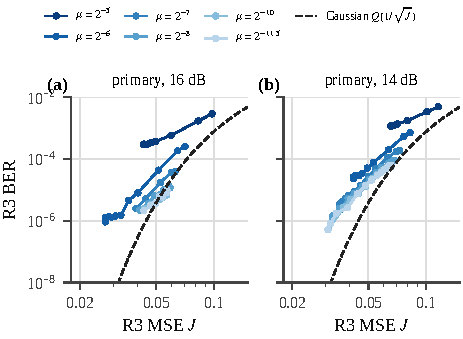
\includegraphics[width=\linewidth]{figs/bermse.pdf}
\caption{\nb{R3 BER against R3 MSE on the primary channel (\lvl{L1}, 100 seeds; points with at least 20 errors). Each line is one step size, traced over the variation rates (slow at the left, fast at the right). Dashed: the Gaussian prediction \eqref{eq:bergauss}. For a fixed $\mu$, BER rises with MSE; across step sizes, equal MSE does not mean equal BER.}}
\label{fig:bermse}
\end{figure}

\begin{figure*}[t]
\centering
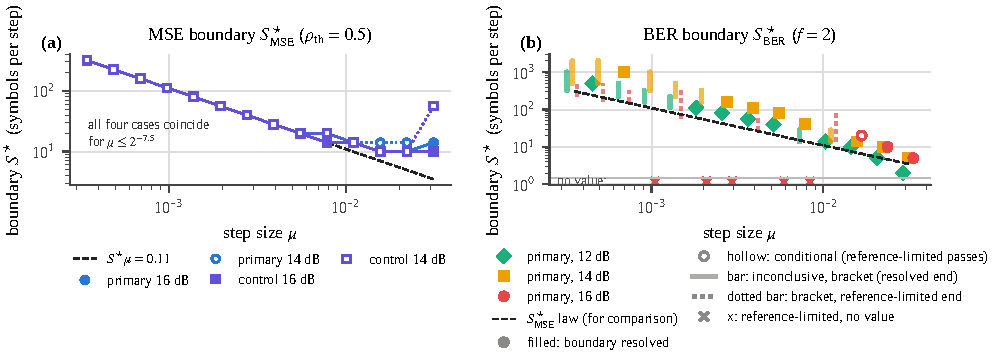
\includegraphics[width=\linewidth]{figs/boundaries.pdf}
\caption{\nb{Tracking boundaries against step size, primary and control channels (\lvl{L1}, supervised, 100 seeds; 1500 at 14\,dB for $\mu\le2^{-7}$). $S$ is the number of symbols between channel changes, so a larger $S^\star$ means the receiver already loses tracking at a slower channel. (a)~$S^\star_{\rm MSE}$, the fastest grid rate at which the tracking loss is statistically below 0.5: for $\mu\le2^{-7.5}$ all four cases coincide on $S^\star\mu\approx0.11$, i.e.\ halving $\mu$ doubles the required $S$. (b)~$S^\star_{\rm BER}$ ($f=2$) on the primary channel at 12, 14 and 16\,dB, with every outcome shown: filled marker, boundary resolved; hollow marker, conditional (passes limited by the measurable reference); bar, boundary point statistically inconclusive, so only the bracket between the last pass and the first failure is known (dotted when the pass end is reference-limited); $\times$, no value can be claimed because the reference BER is too small to measure. The BER boundary lies at slower variation than the MSE boundary and moves further as the SNR rises.}}
\label{fig:bound}
\end{figure*}

\begin{table*}[t]
\centering\small
\caption{\nb{Tracking boundaries (\lvl{L1}, 100 seeds). $S^\star_{\rm MSE}$ ($\rho_{\rm th}=0.5$) and $S^\star_{\rm BER}$ ($f=2$, primary channel). u: $\rho$ undefined. n.d.\ [a, b]: boundary point inconclusive, transition between $S=a$ and $S=b$. R: resolved; C: conditional (reference-limited passes). Half-power step sizes follow the same pattern (full tables in the code package).}}
\label{tab:sstar}
\color{blue}
\setlength{\tabcolsep}{4pt}
\begin{tabular}{@{}l|ccccc|ccc@{}}
\toprule
& \multicolumn{5}{c|}{$S^\star_{\rm MSE}$} & \multicolumn{3}{c}{$S^\star_{\rm BER}$, primary}\\
$\mu$ & prim.\ 16 & prim.\ 14 & prim.\ 12 & ctrl.\ 16 & ctrl.\ 14 & 12\,dB & 14\,dB & 16\,dB\\
\midrule
$2^{-5}$ & 14 & u & u & 10 & 56 & 2 (R) & 5 (R) & 5 (R)\\
$2^{-6}$ & 10 & 14 & 14 & 10 & 10 & 10 (R) & 14 (R) & 20 (C)\\
$2^{-7}$ & 20 & 20 & 20 & 14 & 20 & n.d.\ [28, 14] & 40 (R) & ref.-limited\\
$2^{-8}$ & 28 & 28 & 28 & 28 & 28 & 56 (R) & 112 (R) & n.d.\ [56, 28]\\
$2^{-9}$ & 56 & 56 & 56 & 56 & 56 & 112 (R) & n.d.\ [320, 160] & ref.-limited\\
$2^{-10}$ & 112 & 112 & 112 & 112 & 112 & n.d.\ [320, 160] & n.d.\ [1000, 320] & ref.-limited\\
$2^{-11}$ & 224 & 224 & 160 & 224 & 224 & 500 (R) & n.d.\ [2000, 500] & n.d.\ [500, 160]\\
\bottomrule
\end{tabular}
\end{table*}

\noindent\textbf{Usefulness against the controls ($S_{\rm cross}$).} The PPR asked where the adaptive receiver ceases to outperform its controls, and expected that R2 might match or beat R3 under very slow variation. \nb{On the primary channel R3's BER advantage over both R1 and R2 is demonstrated at \emph{every} $S$ down to $S=1$, for all $\mu\le2^{-6}$ at 12, 14 and 16\,dB. A loss of advantage is confirmed only for $\mu=2^{-5}$ at $S\le2$, where R3's gradient noise is largest. One point, $\mu=2^{-5.5}$ at 16\,dB and $S=1$, is inconclusive (BER $8.30\times10^{-4}$ for R3 against $8.01\times10^{-4}$ for R2); no significant advantage is demonstrated there and no equivalence is claimed. On the control channel at 16\,dB most points are inconclusive because all three receivers make almost no errors. R3 therefore loses tracking \emph{accuracy} ($\rho>0.5$) long before it stops being \emph{useful}: losing half of the tracking margin still leaves a lagging filter that is much closer to the moving optimum than a filter frozen at the training channel (R2) or no filter at all (R1), whose errors are set by the full channel mismatch (\cref{fig:traj}). R2 never matched R3 on the primary channel, because even a slow triangle sweeps the whole channel range, away from R2's training state.}

\subsection{P4: the optimum step size}
\label{sec:muopt}
The step-size study tests the prediction \eqref{eq:mis} of an interior optimum that grows with the variation rate. \nb{For every $S$ an interior optimum $\mu_{\rm opt}$ exists and grows with $1/S$ (\cref{fig:muopt}a). The fitted exponent ${\rm d}\log_2\mu_{\rm opt}/{\rm d}\log_2(1/S)$ is 0.519, 0.525 and 0.511 on the primary channel (16/14/12\,dB) and 0.593 and 0.575 on the control channel (16/14\,dB). The seed-only 95\,\% interval is $\pm0.0005$; the real uncertainty is the systematic band over seven pre-declared fit variants, about $\pm0.03$ (e.g.\ 0.487--0.543 at 16\,dB; error bars in \cref{fig:muopt}b). The exponent is channel-dependent and lies between the random-walk 1/2 and the steady-ramp 2/3, and its local slope changes along $S$. The PPR's square-root prediction happens to describe the primary channel; \cref{sec:theory} shows why, and that this is not evidence of random-walk behaviour.}

\begin{figure*}[t]
\centering
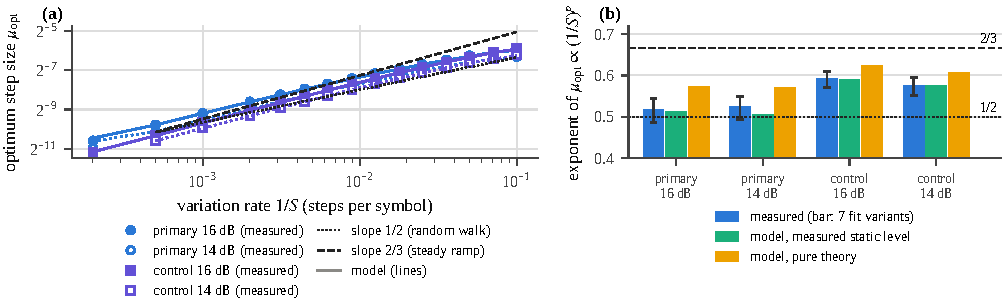
\includegraphics[width=\linewidth]{figs/muopt.pdf}
\caption{Optimum step size against the variation rate (\lvl{L1}, supervised, 100 seeds). (a)~Measured $\mu_{\rm opt}$ (markers) for both channels at 14 and 16\,dB, \nb{the theory model of \cref{sec:theory} (lines)}, and reference slopes 1/2 and 2/3 (their vertical position is arbitrary; only the slope matters). \nb{(b)~Fitted exponent $p$: measured (error bar: range over seven pre-declared fit variants, the dominant uncertainty), model with the measured static level, and pure first-order theory. The primary-channel exponent (0.52) is consistent with 1/2 within its uncertainty; the control-channel exponent (0.58--0.59) lies between 1/2 and 2/3. The model with the measured static level reproduces both within 0.02.}}
\label{fig:muopt}
\end{figure*}

\subsection{Coefficient trajectories}
\label{sec:traj}
The PPR planned to overlay the LMS coefficients on the known optimum trajectory (\cref{fig:traj}). \nb{At $S=1000$ the filter follows (relative rms coefficient error 0.022) with a lag of about 950--1300 symbols; at $S=1000$ the lag scales as $1/\mu$ (168, 400, 1072, 1952, 3440 symbols for $\mu=2^{-6}\ldots2^{-10}$, log--log slope $-1.10$). At $S=56$, twice the boundary, the coefficient swing shrinks to 64--73\,\% of the optimum's (error 0.16); at $S=14$, half the boundary, to 28--39\,\% (error 0.26): the filter traces a delayed, shrunken copy of the optimum. This is what the boundary means physically.}

\begin{figure*}[t]
\centering
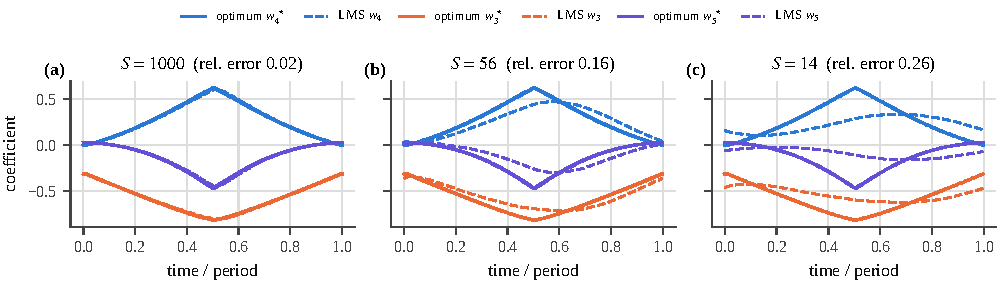
\includegraphics[width=\linewidth]{figs/traj.pdf}
\caption{The three most-moving coefficients over one period: exact moving optimum (solid) and LMS (dashed, mean of 20 seeds), $\mu=2^{-8}$, 16\,dB (\lvl{L1}). \nb{(a)~$S=1000$: LMS follows. (b)~$S=56$ and (c)~$S=14$ ($S^\star_{\rm MSE}=28$): LMS lags and its swing shrinks.}}
\label{fig:traj}
\end{figure*}

\subsection{Triangle against sinusoid}
\label{sec:trisin}
The PPR chose a triangular trajectory because it needs no sine hardware, and committed to checking in floating point that the triangle and a sinusoid give comparable tracking at matched average rates of change. \nb{A sinusoid with the same extremes, start point and period has the same average rate $|{\rm d}a/{\rm d}n|=2^{-7}/S$ but a peak rate $\pi/2$ times larger. Over $S=1000\ldots5$, three step sizes and 20 seeds (\cref{fig:trisin}), the two give the same kind of tracking curve, but at matched average rate the sinusoid is harder: R3's excess MSE is 5--36\,\% higher and, where tracking dominates, the sinusoid behaves like a triangle running 1.2--1.6 times faster. Matched at \emph{peak} rate, the two agree within $-24\ldots+34$\,\% over most of the range. Part of the difference is not tracking: the sinusoid dwells longer near the harsh end, which also raises R1's BER ($2.7\to3.9\times10^{-2}$). The two families are therefore comparable when matched at peak rate; at matched average rate the triangle is not a worst case.}

\begin{figure}[t]
\centering
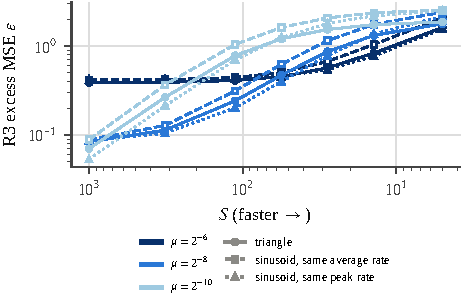
\includegraphics[width=\linewidth]{figs/trisin.pdf}
\caption{Triangle against sinusoid, primary channel, 16\,dB, 20 seeds (\lvl{L1}): R3's oracle-normalised excess MSE $\varepsilon$ against $S$. \nb{At matched average rate the sinusoid is harder; matched at peak rate the curves nearly coincide.}}
\label{fig:trisin}
\end{figure}

\subsection{Decision-directed and pilot-assisted operation}
\label{sec:dd}
The PPR required the decision-directed divergence threshold to be measured and reported, and the supervised results to be checked against realisable modes. \nb{At 14\,dB, for $\mu=2^{-6},2^{-8},2^{-10}$ and all $S$ from 1000 down to 1 (20 seeds), decision-directed, pilot-assisted (one pilot every 10 or 50 symbols) and supervised R3 give the same BER and MSE within statistical noise; R3's own decision error rate there is at most $7.3\times10^{-4}$. \emph{The supervised tracking results above therefore also describe a realisable decision-directed receiver on this channel at 14\,dB for $\mu\le2^{-6}$.} Divergence is set by the step size and the SNR, not by the variation rate (\cref{fig:dd}; $S=28$ and $S=1000$ behave alike): $\mu=2^{-5}$ loses lock at every SNR, $\mu=2^{-6}$ at $\le10$\,dB (1/20 runs at 10\,dB, 8/20 at 8\,dB, 20/20 at 6\,dB), and $\mu\le2^{-7}$ is safe down to 6\,dB. Too short a training also breaks it: forcing the switch after 25--50 training symbols loses lock in 20/20 runs, after 100 symbols in 9--19/20, after $\ge200$ symbols in none. Abrupt jumps $40\leftrightarrow116$ at 6--14\,dB never broke decision-directed adaptation at $\mu=2^{-8}$.}

\begin{figure}[t]
\centering
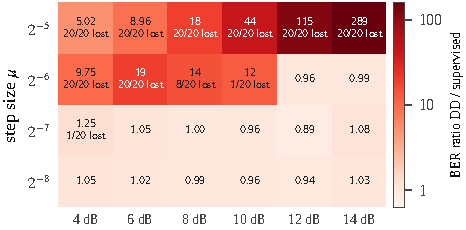
\includegraphics[width=\linewidth]{figs/dd.pdf}
\caption{Decision-directed operation, primary channel, $S=28$, 20 seeds (\lvl{L1}). \nb{Cell: BER of decision-directed R3 divided by supervised R3 on identical data; ``lost'': runs that lost lock. Values near 1 mean decision-directed operation is as good as supervised; the boundary runs diagonally in $(\mu,\mathrm{SNR})$.}}
\label{fig:dd}
\end{figure}
